\setcounter{table}{0}
\renewcommand\thetable{\Alph{section}.\arabic{table}}
\setcounter{figure}{0}
\renewcommand\thefigure{\Alph{section}.\arabic{figure}}
\section{Anatomy of the candidate event}
\label{sec:cand}
The candidate event is an $e\mu + 3$ jets event (run=148864, lumi=225,
event=267767817).  A summary of the objects in the event is given in
Table~\ref{tab:cand1}; event displays are in Figure~\ref{fig:cand1}.

The {\tt ParticleFlow} and {\tt tcMet/JPT} reconstructions of
jets and \met are very consistent. The event shows a clear back
to back topology, as would be expected from a $t\bar{t}$ event
with high $M(t\bar{t})$ (but any statement on the origin of this
event is just a speculation, of course).

\begin{table}[htb]
\begin{center}
\caption{\label{tab:cand1} Summary of the objects in the candidate event.}
\begin{tabular}{|l|c|c|c|c|c|}
\hline
               &  $P_T$ (GeV) & $\eta$  &  $\phi$  &  b-tagged? & value \\ \hline
muon           &   136.       &  0.046  &  -0.206  &            &       \\
electron       &    88        &  0.389  &   2.529  &            &       \\ \hline
Jet 1 (jpt)    &   267        & -0.161  &   2.709  &  Y         &       \\
Jet 2 (jpt)    &    42        &  0.786  &  -0.739  &  N         &       \\
Jet 3 (jpt)    &    40        &  0.192  &  -1.025  &  N         &       \\ 
SumJetPt (jpt) &              &         &          &            & 350 GeV   \\ \hline
Jet 1  (pf)    &   263        & -0.165  &   2.709  &  Y         &       \\
Jet 2  (pf)    &    49        &  0.727  &  -0.723  &  N         &       \\
Jet 3  (pf)    &    34        &  0.117  &  -1.020  &  N         &       \\ 
SumJetPt  (pf) &              &         &          &            & 347 GeV   \\ \hline
tcMET          &   198        &         &  -0.557  &            &       \\ 
pfMET          &   194        &         &  -0.503  &            &       \\ \hline
$P_T(\ell\ell)$&    65        &         &   0.354  &            &       \\
$M(\ell\ell)$  &              &         &          &            & 217 GeV \\
MT2 (tcMet)    &              &         &          &            & 42 GeV  \\
MT2J (tc$+$JPT)&              &         &          &            & 97 GeV  \\
Mass (tc$+$JPT)&              &         &          &            & 159 GeV \\
Meff (tc$+$JPT)&              &         &          &            & 771 GeV \\
\hline
\end{tabular}
\end{center}
\end{table}


\begin{figure}[tbh]
\begin{center}
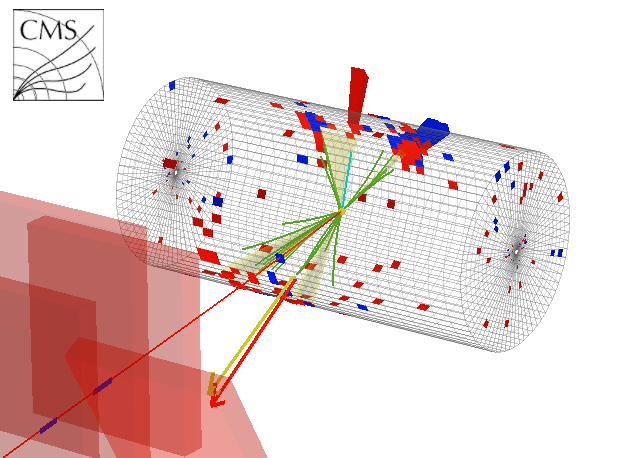
\includegraphics[width=0.6\linewidth]{OSG_3D.png}
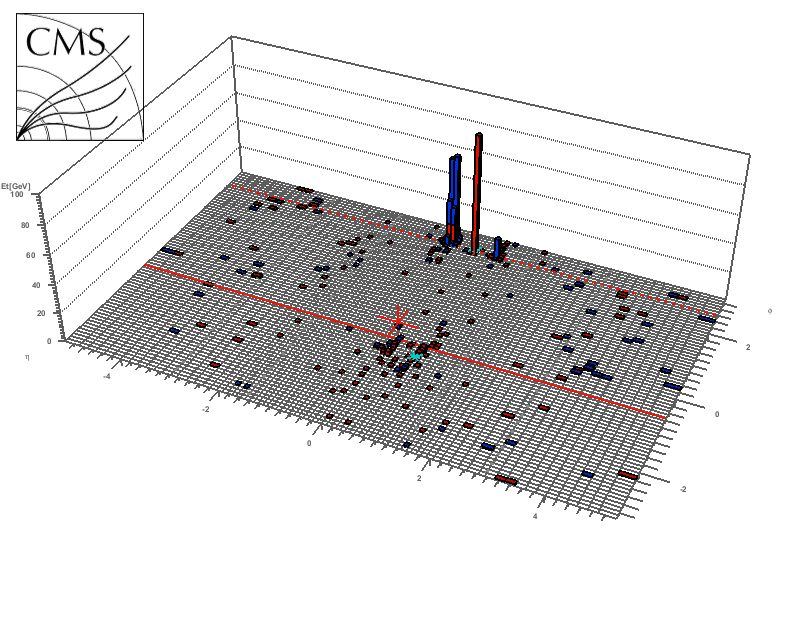
\includegraphics[width=0.6\linewidth]{OSG_lego.png}
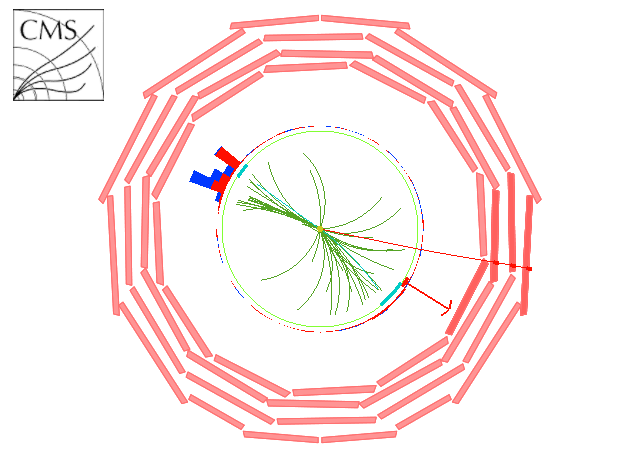
\includegraphics[width=0.6\linewidth]{OSG_rphi.png}
\caption{\label{fig:cand1}Event display for the candidate event.}
\end{center}
\end{figure}

\clearpage
